\documentclass{article}

\usepackage[margin=1in]{geometry}
\usepackage{amsmath}
\usepackage{amsfonts}
\usepackage{amssymb}
\usepackage{amsthm}
\usepackage{polyglossia}
\usepackage{graphicx}
\usepackage{fontspec}
\usepackage{algorithm}
\usepackage{algpseudocode}
\usepackage{listings}
\usepackage[colorlinks=true, linkcolor=black]{hyperref}

\graphicspath{ {./images/} }

\setdefaultlanguage{spanish}
\setmainfont{Latin Modern Roman}

\title{
\includegraphics[scale=0.2]{etsiinf.png}\\[2cm] \textbf{\textit{Rush Hour}.\\Solucionador y clasificador de dificultad de mapas en Haskell.} }
\author{Carmen Toribio Pérez (22M009)\\Marcos Carnerero Blanco (22M039)}
\date{}

\begin{document}

\maketitle

\newpage
\tableofcontents

\newpage
\section{Introducción}
\subsection{\textit{Rush Hour}. Contexto.}
\textit{Rush Hour} es un conocido rompecabezas de bloques deslizantes inventado por Nob Yoshigahara en la década de 1970. El juego consta de un tablero de 6x6 casillas que simula un aparcamiento donde se aparcan coches (que ocupan dos posiciones) y camiones (que ocupan tres). El objetivo es conseguir que uno de los coches (el rojo, siempre en la tercera fila) llegue a la salida, moviendo los otros vehículos. Además, los movimiéntos de los vehículos tienen ciertas restricciones:
\begin{itemize}
  \item Un movimiento supone desplazar un vehículo en línea recta tantas posiciones como se desee. Es decir, si el coche está en horizontal, a la izquierda o a la derecha; y si el coche está en vertical, arriba o abajo.
  \item Los vehículos no pueden rotar ni atravesar otros vehículos.
  \item Los vehículos no pueden salir del aparcamiento.
\end{itemize}

\begin{center}
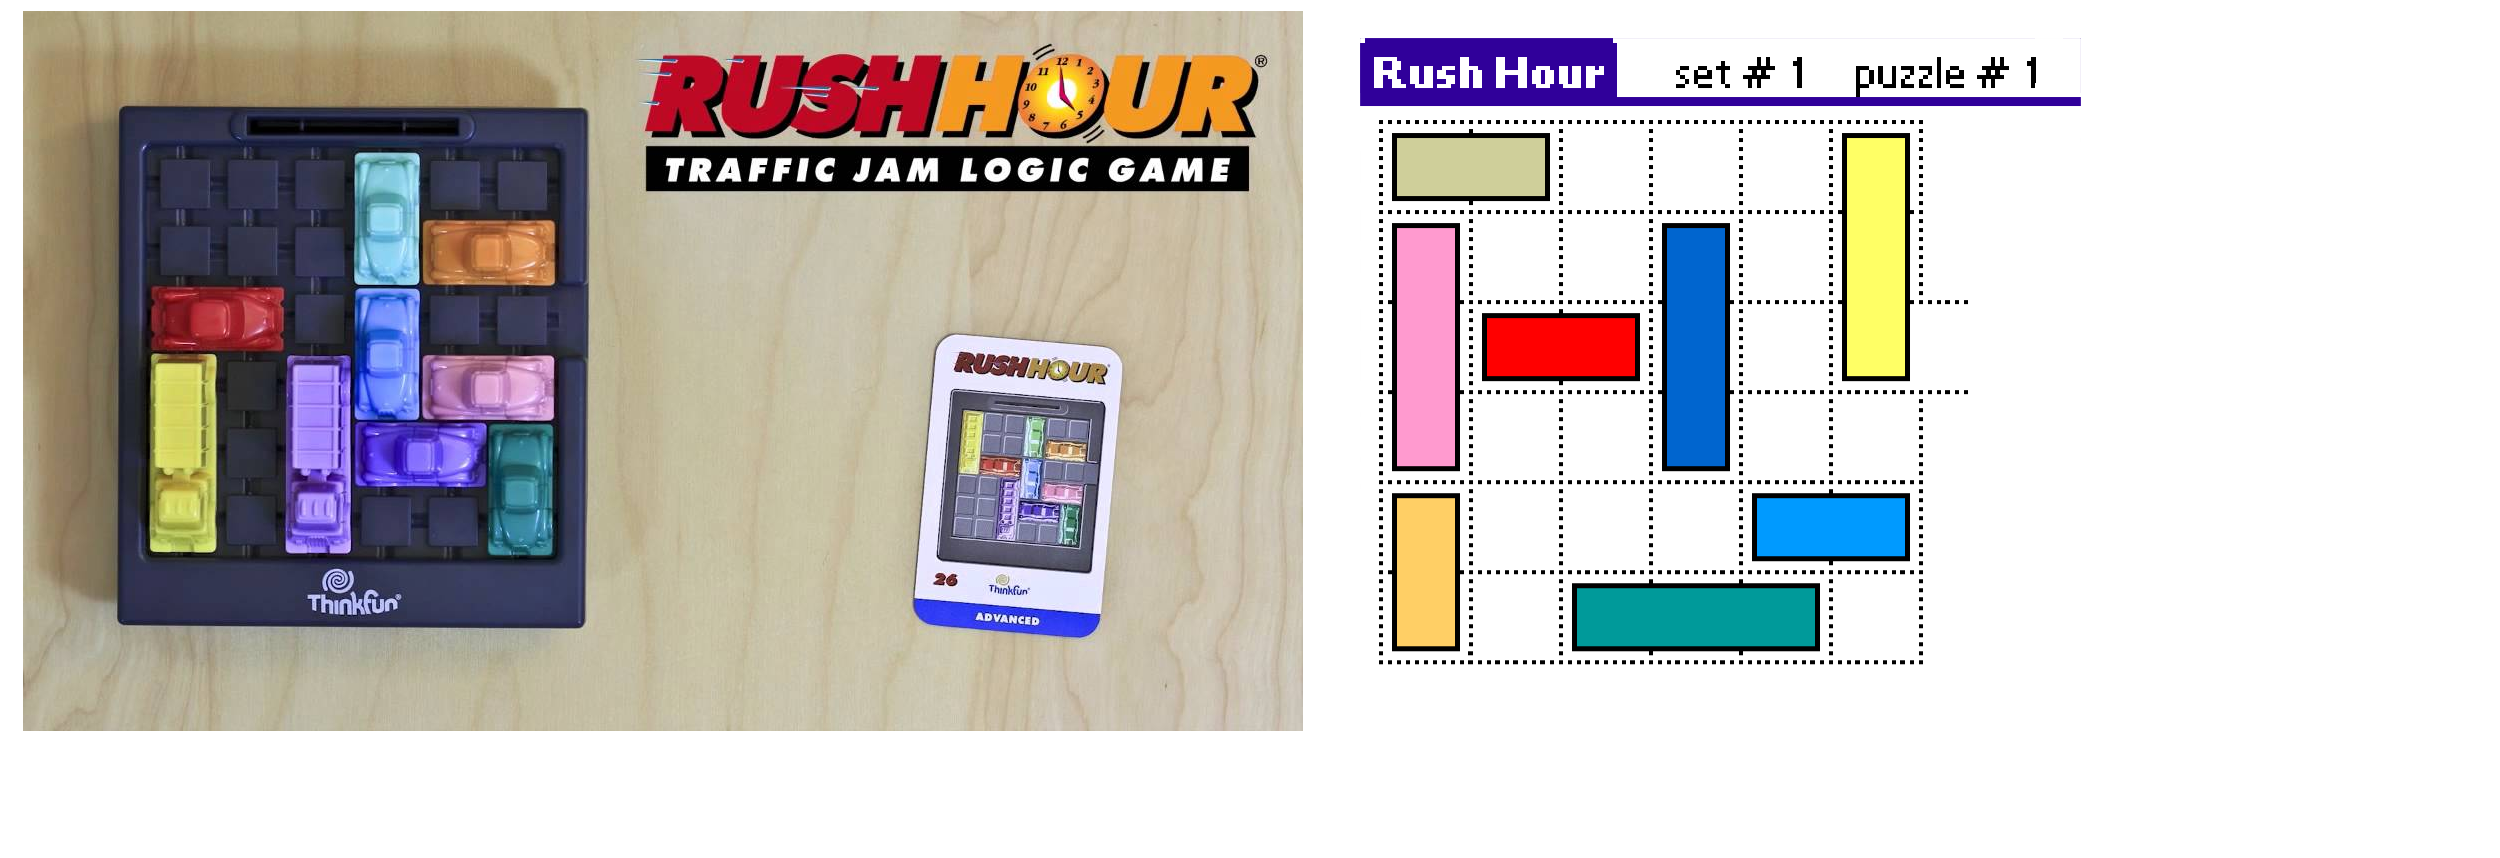
\includegraphics[scale=0.35]{images/rushhour.png}
\end{center}

\subsection{Objetivo de la práctica.}
El objetivo de esta práctica consiste en desarrollar un clasificador de dificultad de mapas de \textit{Rush Hour}. Para ello:

\begin{itemize}
  \item Se ha desarrollado un programa que resuelve mapas de manera óptima utilizando el algoritmo A*, encontrando el mínimo número de movimientos necesarios.
  \item Se ha propuesto una fórmula explicada con detalle en la \textbf{\hyperref[sec:sec3]{sección 3}} que, considerando varios factores,clasifica los mapas en 4 niveles: principiante (\textit{beginner}), intermedio (\textit{intermediate}), avanzado (\textit{advanced}) y experto (\textit{expert}).
\end{itemize}

\newpage

\section{Algoritmo A*.}
El algoritmo A* es una técnica de búsqueda de ruta que encuentra el camino más corto entre un punto de partida y un destino en un grafo ponderado. Utiliza una función heurística para estimar la distancia al destino, lo que hace que sea más eficiente que otros algoritmos de búsqueda como BFS (búsqueda en amplitud) o DFS (búsqueda en profundidad).\\

A* combina la búsqueda por costo uniforme y la búsqueda heurística, utilizando una función de evaluación $f(n) = g(n) + h(n)$, donde $g(n)$ es el costo acumulado y $h(n)$ es la función de la heurística. \\

En concreto, en esta práctica:
\begin{itemize}
\item \textbf{Función heurística}: $h(n) = 1 + k$ con $k = $ cantidad de véhiculos bloqueando el camino entre el coche objetivo y la salida, ya que como mínimo será necesario mover el propio coche y los coches que bloquean su camino.
\item \textbf{Costo acumulado}: El coste entre estados siempre será 1, por lo que $g(h) =$ número de movimientos realizados.
\item \textbf{Cola de prioridad}: Usamos un \textbf{Data.Set} que ordenamos según el valor de $f(n)$, para asegurar que siempre procesamos el nodo con menor costo estimado primero.
\end{itemize}

\begin{algorithm}
\caption{Pseudocódigo de A* para \textit{Rush Hour}}
\begin{algorithmic}[]
\State Inicializar algoritmo con el estado inicial del tablero
\While{queden estados por explorar}
    \If{nodo es solución}
        \State \Return camino solución y $g(n)$
    \EndIf
    \For{movimiento válido no visitado previamente}
        \State Generar estados sucesores con los movimientos posibles de los vehículos
        \If{estado no visitado}
            \State Insertar el hijo a la frontera de búsqueda con $f(n) = g(n - 1) + h(n) + 1$, donde $g(n - 1)$ es el costo del padre y $h(n)$ es la heurística del hijo, con un paso más al haber movido un vehículo.
        \EndIf
    \EndFor
\EndWhile
\end{algorithmic}
\end{algorithm}

\section{Calculo de la dificultad.}\label{sec:sec3}

Una vez hallada la solución del tablero, calculamos su dificultad mediante la siguiente fórmula:
\[
0.7 \cdot \text{stepScore}^{1.4} + 0.2 \cdot \sqrt{\text{movedCarsScore}} + 0.1 \cdot \text{simmetryScore}
\]

Donde:
\begin{itemize}
  \item \textbf{stepScore}: número de movimientos necesarios para resolver el tablero, obtenido directamente del algoritmo A*.
  \item \textbf{movedCarsScore}: proporción de coches (\(\%\)) que se han movido al menos una vez durante la resolución.
  \item \textbf{simmetryScore}: grado de simetría del tablero, medido como el porcentaje de coches en posiciones simétricas respecto a uno de los ejes.
\end{itemize}

\paragraph{Justificación de la forma de la función}
\begin{itemize}
  \item El factor \(0.7\) y la potencia \(1.4\) sobre \(\text{stepScore}\) introducen una penalización \emph{supralineal}: a mayor número de pasos, la dificultad crece más rápido que linealmente. De este modo, soluciones muy largas reciben un castigo significativamente mayor que las moderadas.
  \item El factor \(0.2\) y la aplicación de la raíz cuadrada sobre \(\text{movedCarsScore}\) atenúan la variación en el número de coches movidos. Esto evita que un pequeño aumento en coches movidos se traduzca en un salto excesivo de dificultad, haciendo la curva de penalización más suave.
  \item El factor \(0.1\) sobre \(\text{simmetryScore}\) suma un componente lineal que recompensa tableros más simétricos (menos coches fuera de espejo), reflejando que la simetría suele facilitar la resolución.
\end{itemize}

\noindent
En conjunto, esta combinación de \emph{pesos} y \emph{transformaciones no lineales} (potencia mayor que 1 para enfatizar valores altos, raíz cuadrada para suavizar) permite calibrar con flexibilidad la importancia relativa de cada métrica en el nivel de dificultad final.

\section{Visualización del tablero.}

Para complementar la práctica y hacerla más atractiva visualmente, hemos implementado un módulo que muestra el tablero en una ventana emergente. Esto no solo mejora la experiencia del usuario, sino que también facilita la verificación visual de que la solución propuesta es correcta.\\

\begin{center}
  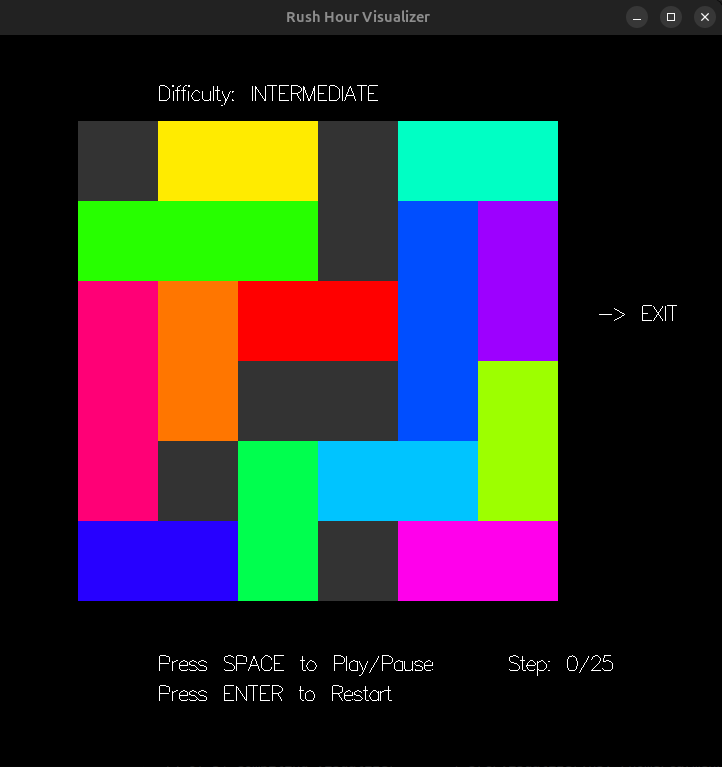
\includegraphics[scale=0.3]{visualizer1.png} \hspace{1cm}
  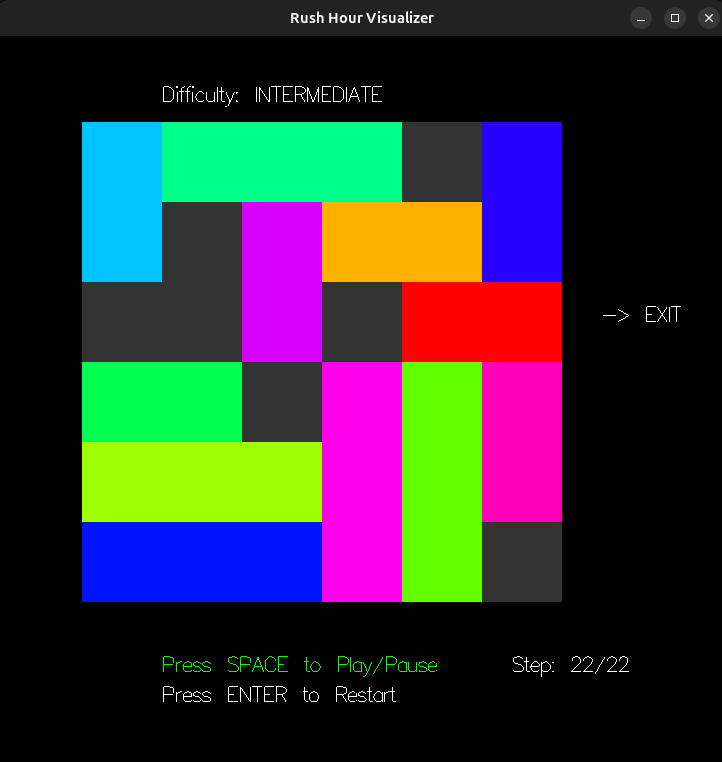
\includegraphics[scale=0.3]{visualizer2.png}
\end{center}

Para lograr esta visualización, se ha utilizado la librería \texttt{Gloss}.\\

Además, la interfaz no solo muestra el tablero, sino que incluye funcionalidades como iniciar o pausar la animación de la solución, reiniciarla y mostrar el paso actual.\\

En cuanto a la selección de colores, se ha implementado un método que asigna un color distinto a cada letra del abecedario, distribuyéndolos homogéneamente a lo largo del círculo cromático de forma no lineal. Se han evitado los tonos cercanos al rojo, ya que este color está reservado exclusivamente para el coche que debe salir del tablero.

\newpage
\section{Librerías usadas.}

Hemos utilizado varias librerías de Haskell que han facilitado el desarrollo del sistema, tanto en la visualización como en la gestión eficiente de los datos.

\subsection{Librería gráfica: Gloss}

Para facilitar la visualización del tablero y la animación de los movimientos, hemos empleado la librería \texttt{Gloss}. Esta librería permite crear gráficos de forma sencilla y eficiente, lo que la hace ideal para simulaciones como la nuestra. La hemos utilizado principalmente para:

\begin{itemize}
  \item \textbf{Visualización del tablero}: Nos permite representar el estado del tablero de forma gráfica, mostrando los vehículos con distintos colores y su disposición sobre el mapa.
  
  \item \textbf{Animación de movimientos con \texttt{animate}}: Actualizamos el estado del tablero cada medio segundo, visualizando cómo se mueven los vehículos hasta alcanzar la solución.
  
  \item \textbf{Interfaz de usuario con controles básicos}: Permite pausar, reiniciar y salir del juego mediante teclas, mejorando así la experiencia del usuario.
\end{itemize}

Aunque esta librería no permite incorporar atajos de teclado más complejos ni acceder al portapapeles (lo que hubiese sido útil, por ejemplo, para introducir el mapa directamente desde la interfaz), su facilidad de uso y su integración con Haskell nos hicieron decantarnos por ella.

\subsection{Librería de estructuras: \texttt{Data}}

Dada la complejidad del proyecto, era necesario gestionar de forma eficiente los estados del tablero y las posiciones de los vehículos. Para ello, hemos utilizado varias estructuras de datos proporcionadas por el módulo \texttt{Data} de Haskell:

\begin{itemize}
  \item \texttt{Data.Map}: Para representar los estados del tablero, analizarlos, almacenarlos y pasarlos como argumentos.
  
  \item \texttt{Data.Set}: Para gestionar las posiciones ocupadas por los vehículos.
  
  \item \texttt{Data.List}: Para la manipulación de listas y la generación de movimientos válidos, con funciones como \texttt{find}.
\end{itemize}

\section{Estructura general del programa.}
\subsection{Módulos}
Los módulos del proyecto están organizados de la siguiente manera:

\begin{table}[h!]
\centering
\begin{tabular}{|l|l|}
\hline
\textbf{Módulo} & \textbf{Función} \\
\hline
AStar & Implementación genérica del algoritmo A*\\
BoardUtils & Definición de tipos, parser de los mapas y cálculo de movimientos posibles del tablero \\
Difficulty & Cálculo de la dificultad del tablero dada una solución\\
Visualizer & Renderizado del mapa con Gloss y bucle de servicio \\
Main & Instanciación de métodos específicos para A* como la heurística e inicialización de la \\
     & ejecución del programa\\
\hline
\end{tabular}
\end{table}

\subsection{Tipos declarados.}

En cada módulo hemos definido los tipos necesarios para representar el estado del tablero, los vehículos y las métricas de dificultad. Hemos utilizado varios \texttt{type} para mejorar la legibilidad y el mantenimiento del código, mientras que los \texttt{data} se han empleado principalmente como si fueran \emph{structs} de C, agrupando en un solo tipo toda la información relevante para los cálculos del módulo correspondiente.\\

A continuación, mostramos la implementación de los tipos declarados:
\begin{lstlisting}[language=Haskell]
-- Módulo: BoardUtils

type Position = (Int, Int) -- (fila, columna)

data Orientation = Horizontal | Vertical deriving (Eq, Ord)

data Car = Car
  { carId :: Char, -- Identificador del coche (A-Z)
    positions :: [Position], -- Lista de posiciones ocupadas por el coche
    orientation :: Orientation -- Orientación del coche (Horizontal o Vertical)
  }
  deriving (Eq, Ord)

type Board = [Car] -- Lista de coches en el tablero

module Difficulty where

data SolutionMetrics = SolutionMetrics
  { steps :: Int, -- Número de movimientos en solución óptima
    movedCars :: Int, -- Cantidad de coches diferentes movidos
    carCount :: Int, -- Cantidad total de coches en el tablero
    symmetryScore :: Int -- Grado de simetría (0-100)
  }
  deriving (Show)

---------------------------------------------------------------------------

-- Módulo: Visualizer

type Step = Int

data World = World
  { steps :: [Board] -- Lista de tableros que representan los pasos de la solución
  , current :: Step -- Índice del paso actual en la lista de pasos
  , playing :: Bool -- Indica si el visualizador está en modo "play"
  , difficultyLabel :: String -- Etiqueta de dificultad del tablero
  }
\end{lstlisting}

\newpage
\section{Posibles mejoras y optimizaciones}

Dada la naturaleza de la práctica, hemos optado por una solución funcional básica, priorizando la claridad y la facilidad de implementación. No obstante, hemos identificado diversas áreas susceptibles de mejora y optimización:

\begin{itemize}
  \item \textbf{Optimización de la heurística}: La heurística actual es sencilla y no considera la disposición de vehículos que, aunque no bloqueen directamente al coche objetivo, sí limitan su movilidad de forma indirecta.
  
  \item \textbf{Paralelización de la búsqueda}: Dado que el algoritmo A* explora múltiples nodos en cada iteración, sería posible diseñar una versión paralela que aproveche mejor los recursos computacionales, especialmente en sistemas multinúcleo.
  
  \item \textbf{Mejora de la visualización}: Se podrían incorporar controles avanzados, como avanzar/retroceder paso a paso por la solución o permitir la interacción directa con el tablero para probar movimientos manuales.
  
  \item \textbf{Optimización de la gestión de estados}: El uso de estructuras más eficientes, como \texttt{tries} o tablas hash, podría reducir significativamente el coste de exploración en tableros complejos con gran número de estados.
  
  \item \textbf{Generación de tableros aleatorios}: Implementar un generador de niveles con dificultad controlada permitiría evaluar automáticamente el rendimiento del sistema y probarlo con una mayor variedad de configuraciones.
  
  \item \textbf{Mejora de la interfaz de usuario}: Una interfaz gráfica más completa permitiría, por ejemplo, cargar tableros desde archivo, introducirlos manualmente o incluso compartirlos mediante un identificador único.
\end{itemize}

\section{Conclusiones}

El sistema desarrollado permite calcular de forma consistente la dificultad de un tablero utilizando una solución óptima obtenida mediante el algoritmo A*, lo que demuestra la aplicabilidad de algoritmos heurísticos en problemas de planificación y búsqueda.\\

Las estructuras inmutables de Haskell han resultado ventajosas para gestionar el estado de forma segura, aunque han exigido técnicas específicas de optimización para mantener un buen rendimiento. El paradigma funcional, con su enfoque en la composición y las funciones de orden superior, ha facilitado una modelización concisa y expresiva del problema.\\

Además, la visualización mediante la librería \texttt{Gloss} ha contribuido a mejorar la experiencia de usuario, permitiendo observar en tiempo real el proceso de resolución del tablero.\\

En conjunto, consideramos que el sistema cumple satisfactoriamente los objetivos planteados y ofrece una base sólida para futuras extensiones.\\

\end{document}
